\documentclass{article}
\usepackage[utf8]{inputenc}
\usepackage{hyperref}
\usepackage{biblatex}
\addbibresource{sample.bib}
\usepackage{todonotes}
\usepackage{graphicx}
\graphicspath{ {imgs/} }
\usepackage{float}
\usepackage{subcaption}
\usepackage{verbatim}

\setcounter{secnumdepth}{3}

\title{TSBK02\\Computer Graphics\\OpenWorld}
\author{Carl Dehlin\\carde650@student.liu.se}
\date{\today}

\begin{document}

\maketitle

\section{Introduction}
This paper is the result of a project in the course Computer Graphics at Linköping University. 
The goal of the project was to investigate techniques for rendering big realistic outdoor environments.
The fundamental goals are listed below.
\begin{itemize}
    \item Realistic camera movement
    \item Automatic terrain generation
    \item Gloss mapping
    \item Environment mapping
    \item Altitude dependent multi-texturing
    \item Sky dome
    \item Simple fog effect
    \item Simple water
    \item Frustum culling
    \item Geomipmapping
\end{itemize}

Techniques for generating large worlds are covered in sections \ref{sec:wgen}, \ref{sec:tex} and \ref{sec:clouds}.
In order to render a big world one needs to compress the information to be displayed.
The solution to this is to limit the amount of vertices being rendered each frame through some kind of
visual surface detection algorithm (VSD) and to limit the resolution of the object being rendered as the level of detail becomes less important (LOD). These topics are covered in sections \ref{sec:VSD} and \ref{sec:LOD}.

In order to make the rendering realistic one has to work a lot with illumination. These topics are covered in section \ref{sec:illumination}.

\section{The large world problem}
In this section techniques concerning rendering big worlds are investigated.

\subsection{World generation} \label{sec:wgen}
In order to generate worlds randomly, one first needs a good random function.
A very good alternative is to utilize the fact that frequencies in nature tends to falloff as $F(\omega) \propto \frac1\omega$.
Generating random frequencies with this distribution and then transforming these to actual spatial coordinates serves as a basis for generating natural shapes such as terrain and clouds.

The terrain height map is generated using a 2D-DFT and the clouds density map with a 3D-DFT (2 spatial, 1 temporal).

\subsection{Texturing} \label{sec:tex}
A natural world needs texturing in order to give the automatically generated shapes any meaning.
Randomly generated terrain does not look like anything special without telling what the different parts represent, for example, texturing the lower parts with green, middle with gray and upper with white will make the random noise look like a mountain.

Texturing according to spatial coordinates only gives a very flat and unrealistic impression, especially for the snow texture as can be seen in figure \ref{fig:snowPlain}. However, using the height-map generated previously and generate snow with probability proportional to the height (normalized between minimum and maximum height, and some morphological operations afterwards) gives the result shown in figure \ref{fig:snowProb}. The corresponding height-map and snow-map are shown in figure \ref{fig:heightMapSnowMap}.

\begin{figure}[H]
\centering
    \begin{subfigure}[b]{0.45\textwidth}
        \centering
        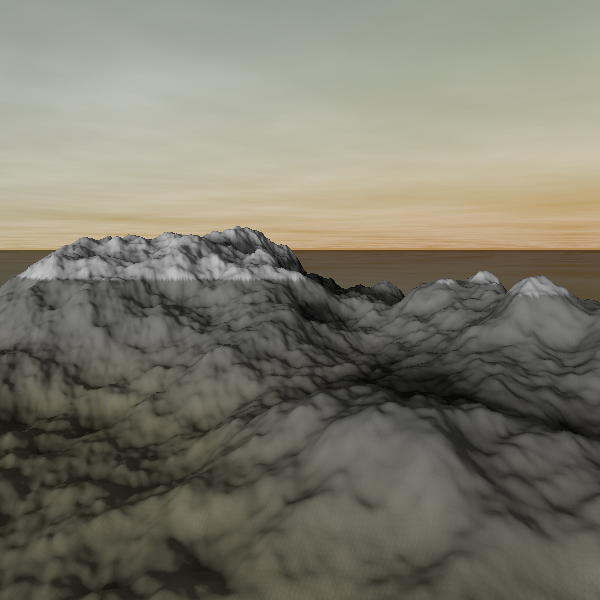
\includegraphics[scale=0.25]{snowPlain}
        \caption{Snow based on terrain height}
        \label{fig:snowPlain}
    \end{subfigure}
    ~
    \begin{subfigure}[b]{0.45\textwidth}
        \centering
        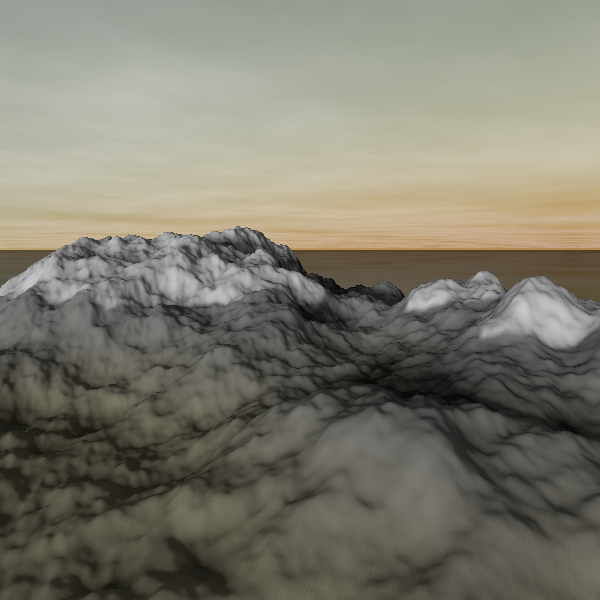
\includegraphics[scale=0.25]{snowProb}
        \caption{Snow based on snow-map}
        \label{fig:snowProb}
    \end{subfigure}
    \caption{}
    \label{fig:snowPlainProb}
\end{figure}

\begin{figure}[H]
\centering
    \begin{subfigure}[b]{0.45\textwidth}
        \centering
        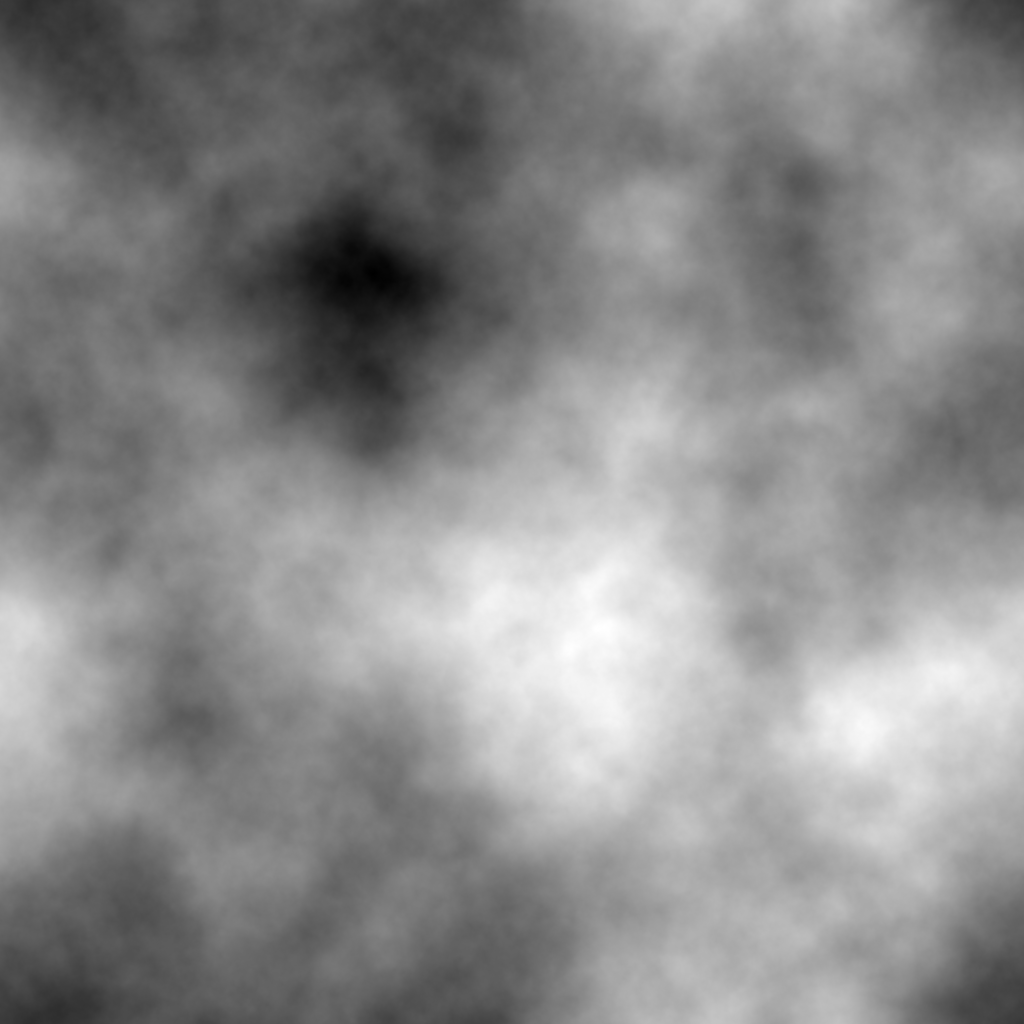
\includegraphics[scale=0.15]{heightMap}
        \caption{Generated height-map}
        \label{fig:heightMap}
    \end{subfigure}
    ~
    \begin{subfigure}[b]{0.45\textwidth}
        \centering
        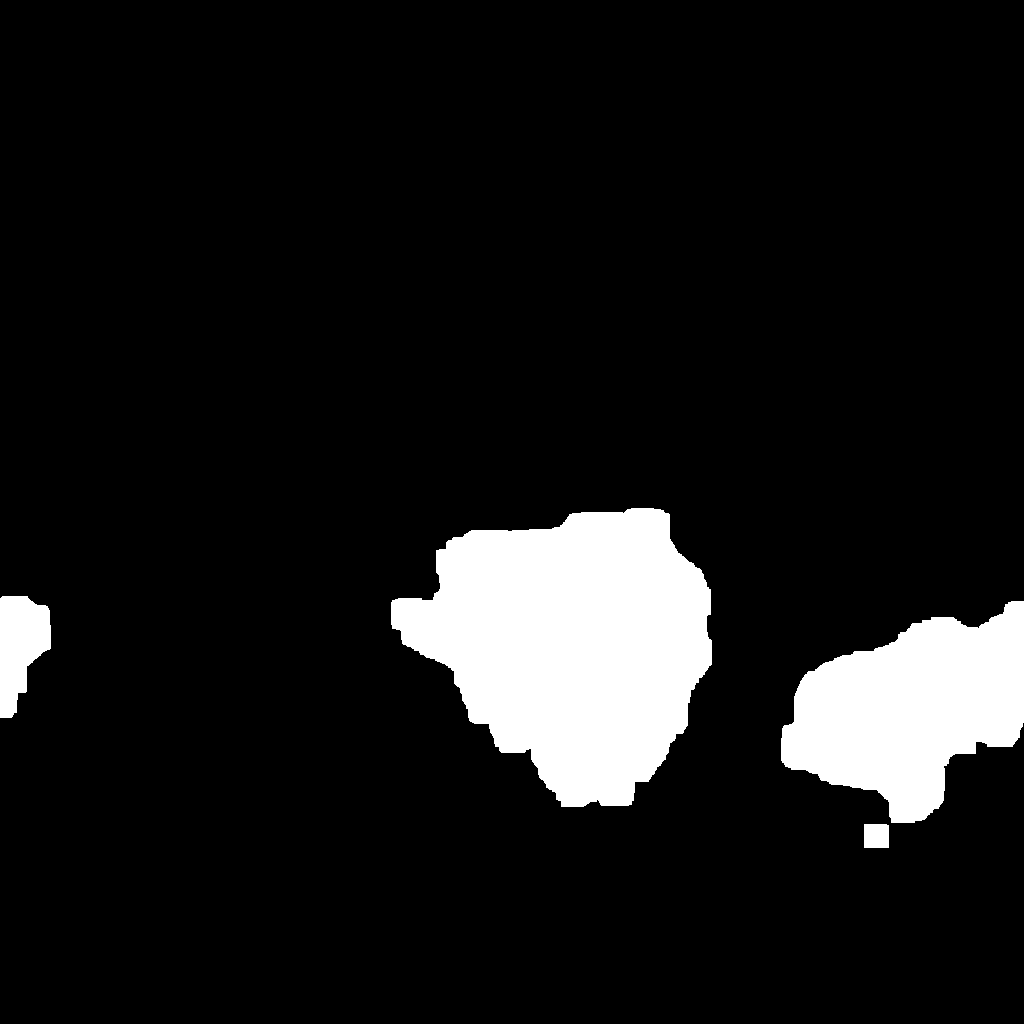
\includegraphics[scale=0.15]{snowMap}
        \caption{Generated snow-map}
        \label{fig:snowMap}
    \end{subfigure}
    \caption{}
    \label{fig:heightMapSnowMap}
\end{figure}

With the height-map, local topology like texture coordinates and tangent space is generated.
The texture coordinates together with the tangent space can be used together with a normal-map and gloss-map to give details to the terrain. The results corresponding to no local detail, with normal-map, with gloss-map and with both is shown in figure \ref{fig:tangentSpaceSnow}. A visualization of the tangent space is shown in figure \ref{fig:tangentSpaceViz}.

\begin{figure}[H]
\centering
    \begin{subfigure}[b]{0.45\textwidth}
        \centering
        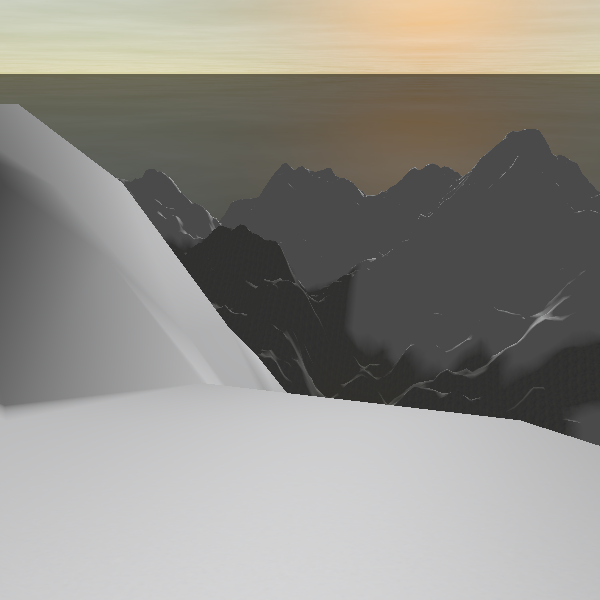
\includegraphics[scale=0.25]{noMap}
        \caption{No local detail}
        \label{fig:noMap}
    \end{subfigure}
    ~
    \begin{subfigure}[b]{0.45\textwidth}
        \centering
        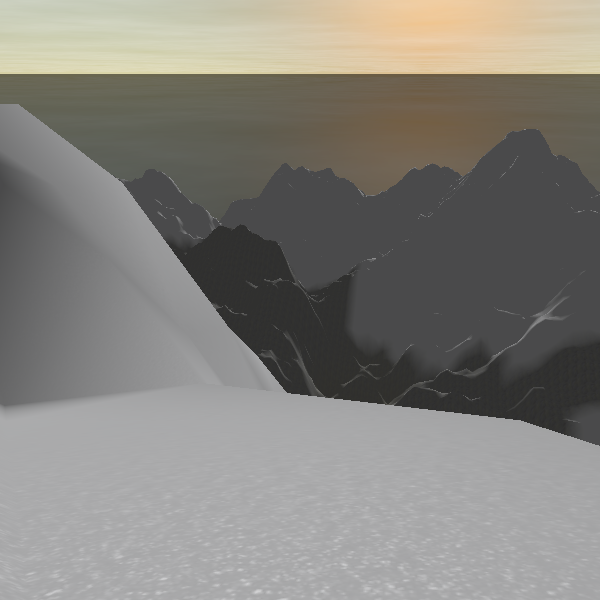
\includegraphics[scale=0.25]{glossMap}
        \caption{With gloss-map}
        \label{fig:glossMap}
    \end{subfigure}
    ~
    \begin{subfigure}[b]{0.45\textwidth}
        \centering
        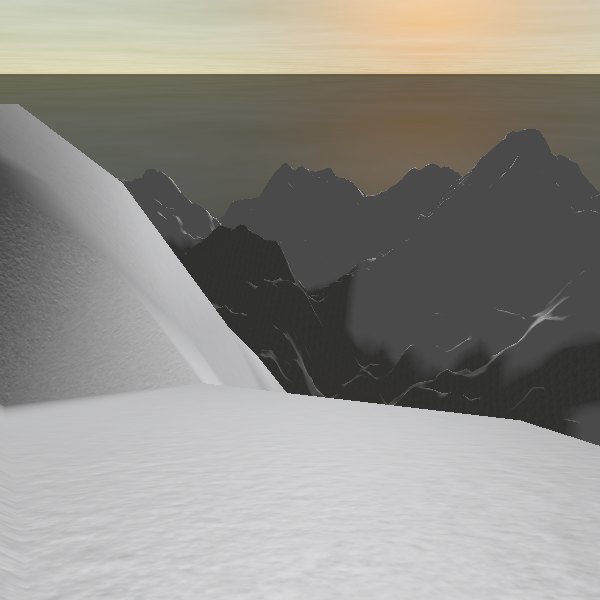
\includegraphics[scale=0.25]{normalMap}
        \caption{With normal-map}
        \label{fig:normalMap}
    \end{subfigure}
    ~
    \begin{subfigure}[b]{0.45\textwidth}
        \centering
        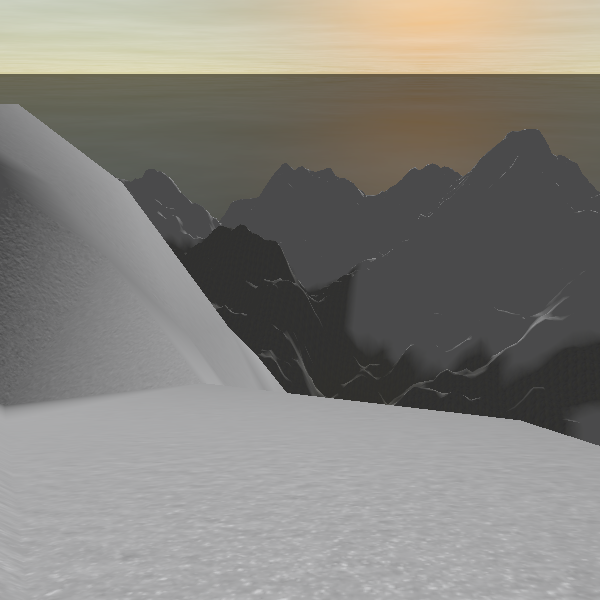
\includegraphics[scale=0.25]{glossNormalMap}
        \caption{With gloss- and normal-map}
        \label{fig:glossNormalMap}
    \end{subfigure}
    \caption{}
    \label{fig:tangentSpaceSnow}
\end{figure}

\begin{figure}[H]
\centering
    \centering
    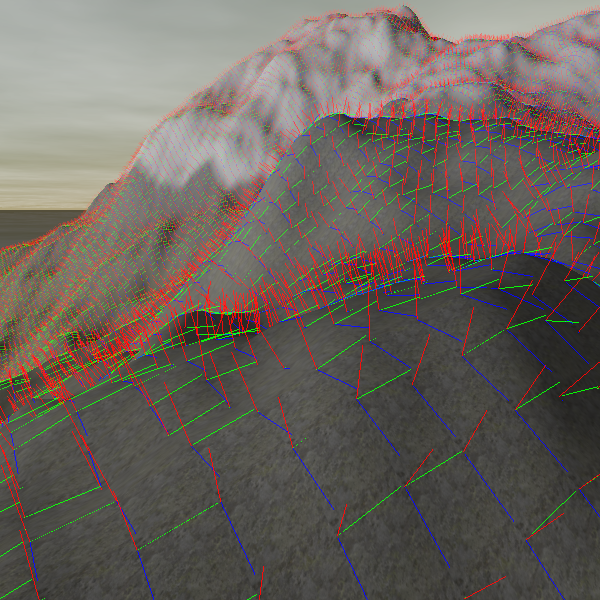
\includegraphics[scale=0.5]{tangentSpaceViz}
    \caption{Visualization of the local topology}
    \label{fig:tangentSpaceViz}
\end{figure}

\subsection{Clouds} \label{sec:clouds}
Rendering clouds to a sky dome is not trivial. Sampling from the cloud texture with the skydome texture coordinates (spherical angles) directly results in a very non-open effect, as can be seen in in figure \ref{fig:cloudPlain}.
The problem clearly lies in the horizon, so a first approach could be to try to hide this effect with a fog, the result can be seen in figure \ref{fig:cloudFog}. This, apart from looking a bit dull, just hides the fundamental error.
The problem is that the coordinates need to be perspective corrected, as can be seen in figure \ref{fig:cloudProj}.
Now the problem is that we can see how the same texture is repeated over and over, so we again try to hide this with a fog effect, the result is quite pleasing and can be seen in figure \ref{fig:cloudProjFog}.

\begin{figure}[H]
\centering
    \begin{subfigure}[b]{0.45\textwidth}
        \centering
        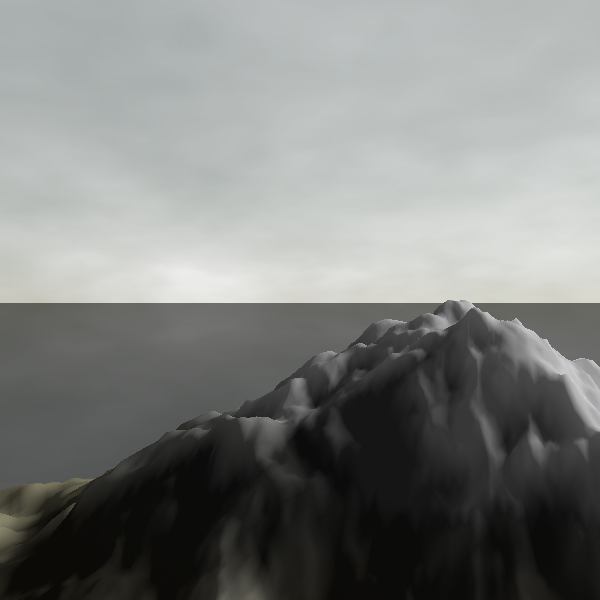
\includegraphics[scale=0.25]{cloudPlain}
        \caption{Clouds with direct texture mapping}
        \label{fig:cloudPlain}
    \end{subfigure}
    ~
    \begin{subfigure}[b]{0.45\textwidth}
        \centering
        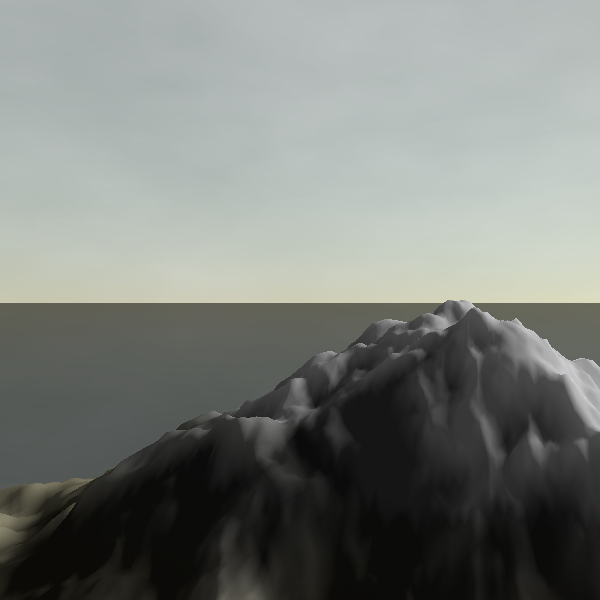
\includegraphics[scale=0.25]{cloudFog}
        \caption{Clouds with horizon fog effect}
        \label{fig:cloudFog}
    \end{subfigure}
    ~
    \begin{subfigure}[b]{0.45\textwidth}
        \centering
        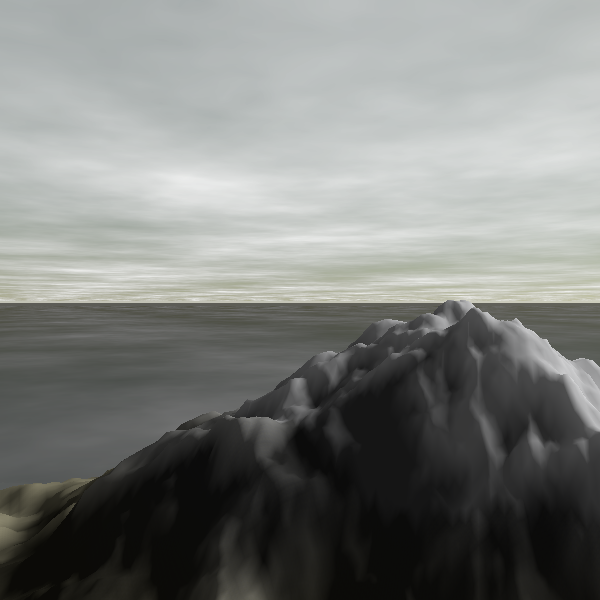
\includegraphics[scale=0.25]{cloudProj}
        \caption{Clouds with perspective corrected texture coordinates}
        \label{fig:cloudProj}
    \end{subfigure}
    ~
    \begin{subfigure}[b]{0.45\textwidth}
        \centering
        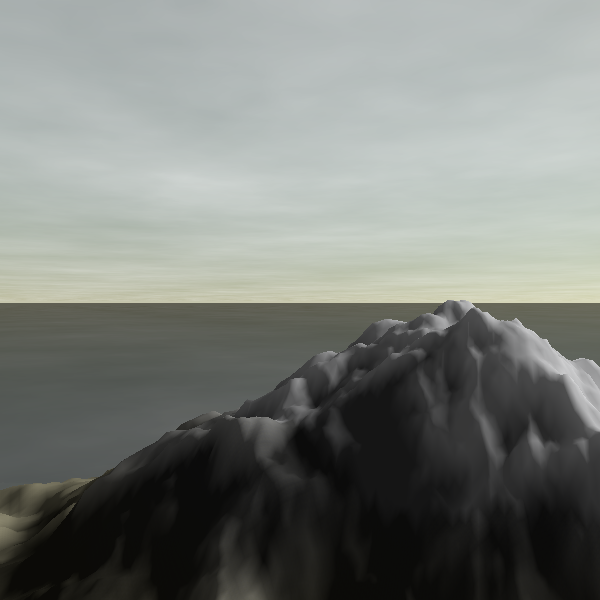
\includegraphics[scale=0.25]{cloudProjFog}
        \caption{Clouds with perspective corrected coordinates and horizon fog effect}
        \label{fig:cloudProjFog}
    \end{subfigure}
    \caption{}
    \label{fig:clouds}
\end{figure}

\subsection{Visual surface detection (VSD)} \label{sec:VSD}
All modern hardware today that supports OpenGL can perform hardware accelerated VSD to some extent.
Atleast it is possible to cull primitives that faces away from the viewer, effectively reducing the amount of fragments by half.
This factor can however be imporoved upon with software accelerated VSD, such as frustum culling, where vertices outside of the camera frustum is skipped in an early stage of the rendering pipeline.

This project implemented a conservative frustum culler, rejecting any object whose bounding box where all vertices are on the same side of the frustum planes.
That is, there are objects that are outside the frustum that passes the VSD test, but no object fails if inside it. %This algorithm is visualized in figure \todo{\ref{fig:frustumCull}}.

\subsection{Level of detail (LOD)} \label{sec:LOD}
VSD is however not sufficient for rendering large worlds, since VSD only gives a constant factor in performance.
What we need is something that scales with the size of the world.
One such approach is geomipmapping, where the resolution of the world decreases as the distance to the object increases.
By reducing the level of detail of objects in the right way this approach actually opens up for possible \emph{infinite} worlds.
If we let $S$ be proportional to the size of the world, $R(D)$ be the resolution at distance $D$, then the total amount of vertices to process is proportional to $V(S)$ according to equation \ref{eq:VSD}.

\begin{equation}
    V(S) \propto \int_S R(D) dD
    \label{eq:VSD}
\end{equation}

Taking the limit of $S$ to infinity, we see that in order for the amount of vertices to be finite the resolution needs to decrease at least as $R(D) \propto \frac{1}{D^\alpha}$, $\alpha > 1$.

However, this is only for the amount of vertices needed to process in the current frame. All vertices still needs to be stored in memory, limiting the size of the world.

For this project, the terrain was generated in multiple scales at powers of 2. The terrain is downscaled by first lowpass filtering with a gaussian kernel, which reduces popping slightly. 
The terrain-mesh is then split into a grid, and for each sub-mesh in the grid we need to constrain the edges to neighboring sub-meshes (since they can have different geomipmap levels when rendered). This is solved similar to the suggested approach given by \cite[13,p.~177]{ingemar}, the reader is referred there for further details.

For each sub-mesh in the grid passing the VSD test, a geomipmap level is chosen according to the distance from the camera to the centroid of the sub-mesh. The geomipmap level is chosen according to equation \ref{eq:geomipmap}. Here, B is the \emph{base resolution}, which is at which distance we should go down a level in resolution, L is the geomipmap level and D the distance to the centroid of the sub-mesh.

\begin{equation}\label{eq:geomipmap}
    L_B(D) = \lfloor \log_2(D / B) \rfloor
\end{equation}

Results for various base resolution levels is shown in figure \ref{fig:geomipmap}.

\begin{figure}[H]
\centering
    \begin{subfigure}[b]{0.45\textwidth}
        \centering
        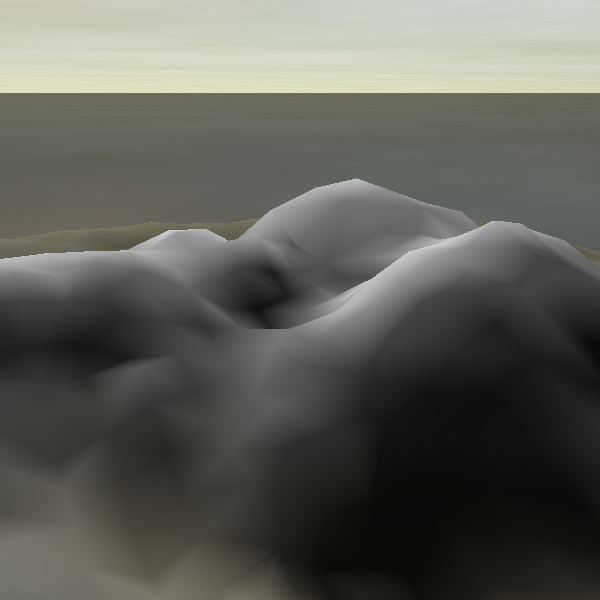
\includegraphics[scale=0.25]{image2}
        \caption{Base resolution 20 meters}
        \label{fig:image2}
    \end{subfigure}
    ~
    \begin{subfigure}[b]{0.45\textwidth}
        \centering
        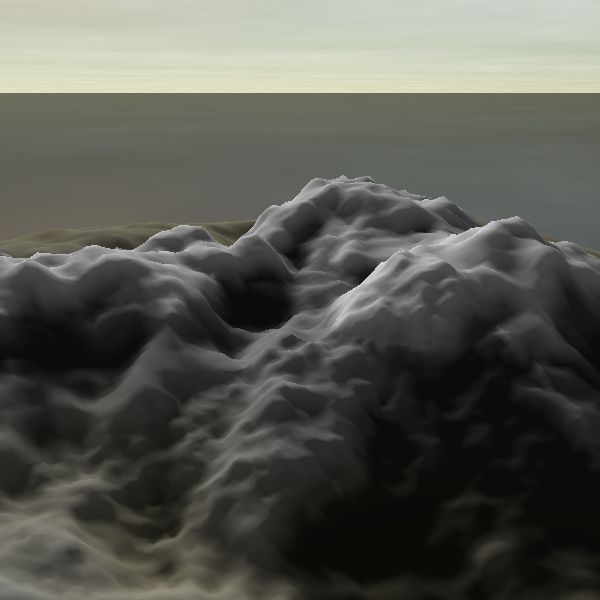
\includegraphics[scale=0.25]{image10}
        \caption{Base resolution 100 meters}
        \label{fig:image10}
    \end{subfigure}
    ~
    \begin{subfigure}[b]{0.45\textwidth}
        \centering
        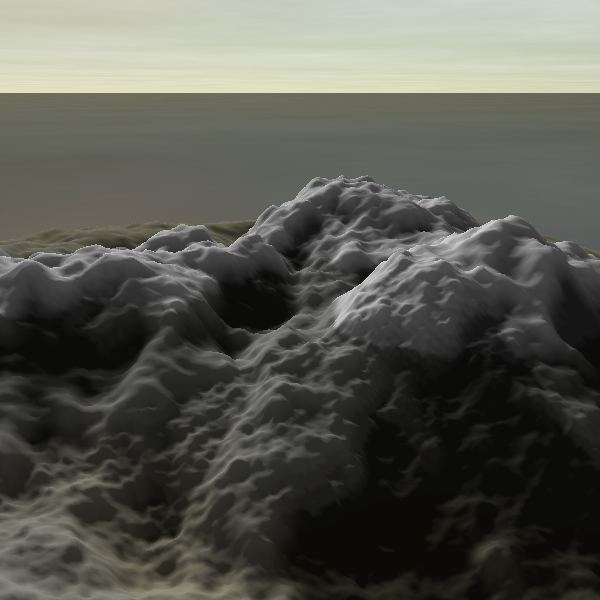
\includegraphics[scale=0.25]{image20}
        \caption{Base resolution 200 meters}
        \label{fig:image20}
    \end{subfigure}
    ~
    \begin{subfigure}[b]{0.45\textwidth}
        \centering
        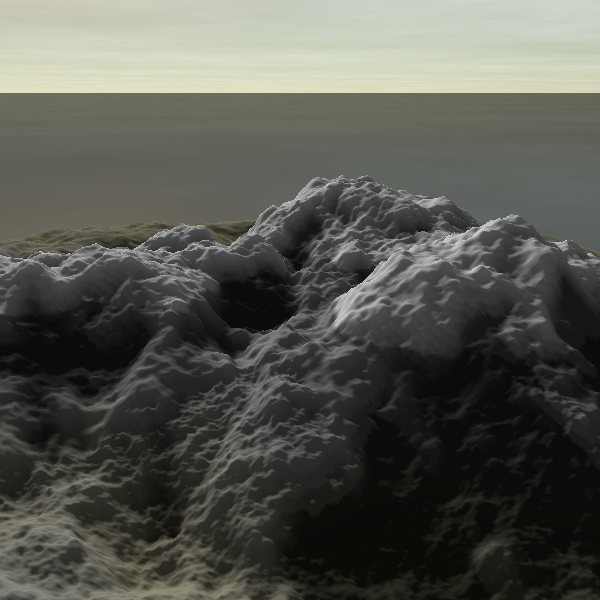
\includegraphics[scale=0.25]{image36}
        \caption{Base resolution 360 meters}
        \label{fig:image36}
    \end{subfigure}
    \caption{Geomipmapping with various base resolution levels}
    \label{fig:geomipmap}
\end{figure}

\section{Illumination (The beautiful world problem)} \label{sec:illumination}
One very important aspect of rendering realistic worlds is illumination.
The human eye is very sensitive to incorrect shading and weird lightning conditions, two of these being sky color and shadows.

\subsection{Sky}
The sky is filled with a spectrum of colors, that varies greatly depending on time and air conditions.
This can be simulated with some kind of ad-hoc gradient over a skydome, however it is very hard to fool the human eye with false colors so a better alternative is to actually simulate the process that makes the sky blue. 
The main process behind this is scattering. Solving the scattering equations is in general a very hard problem, but fast approximations can be enough to give an acceptable result.

A first approximation is to only calculate the first order scattering term, that is, only light rays that have scattered once.
The first order scattering equations are summarized in the out-scattering equation \ref{eq:scattering1} and the in-scattering equation \ref{eq:scattering2}.\cite{nvidia}
Here, $t(a,b,\lambda)$ is the amount of scattered light of wavelength $\lambda$ along the ray from point $a$ to point $b$. $K(\lambda)$ is the Rayleigh scattering coefficient, $S(\lambda)$ is the sun intensity and $F(\lambda)$ is the phase function at wavelength $\lambda$. $h/H_0$ is the normalized height (between 0 and 1) of the current points along the ray. These equations are approximated with nested sums of some fixed step length, the outer sum evaluated for each vertex on the sky dome, and the inner integral evaluated along the points taken from the outer integral to the entry points of sunlight in the atmosphere. This is illustrated in figure \ref{fig:scattering}.

\begin{equation}\label{eq:scattering1}
    t(a,b,\lambda) \propto K(\lambda) \int_a^b \exp(-h/H_0) ds
\end{equation}
\begin{equation}\label{eq:scattering2}
    I(\lambda) = F(\theta) S(\lambda) K(\lambda) \int_a^b \exp(-h/H_0) \exp(-(t(a,p)+t(p,c)) ds
\end{equation}

\begin{figure}[H]
\centering
    \centering
    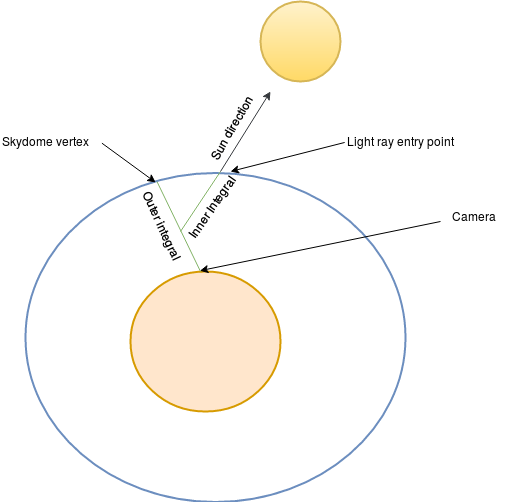
\includegraphics[scale=0.5]{scattering}
    \caption{Illustration of the scattering equations}
    \label{fig:scattering}
\end{figure}

When simulating the scattering equations it is important to do it for many wavelengths, and then combine the results
using a tristimulus model to get the resulting red, green and blue colors. This is because the scattering equations are highly non-linear, and the colors do not blend additively.

This project found that the visible spectrum (400-750 nm) needs to be sampled at least 6 times (linearly spaced samples) in order to approximate the resulting color distribution good enough.
Also, the light rays in both inner and outer integrals needs to be sampled at least 2 times each (linearly spaced samples).

The scattering equations are solved for two phase functions, one for Rayleigh scattering (giving the ambient background colors), and one for Mie scattering (giving the red-yellow colors resulting from larger particles).
The results can be seen in figure \ref{fig:sunScatterResults}.

\begin{figure}[H]
\centering
    \begin{subfigure}[b]{0.45\textwidth}
        \centering
        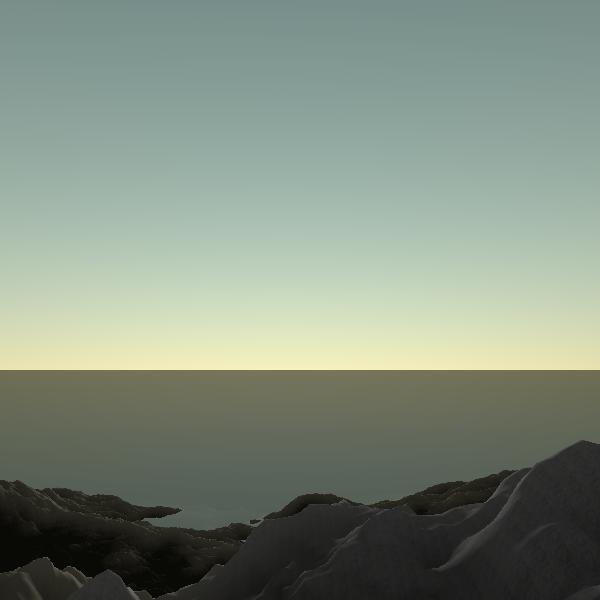
\includegraphics[scale=0.25]{scatterRayleigh}
        \caption{Rayleigh scattering}
        \label{fig:scatterRayleigh}
    \end{subfigure}
    ~
    \begin{subfigure}[b]{0.45\textwidth}
        \centering
        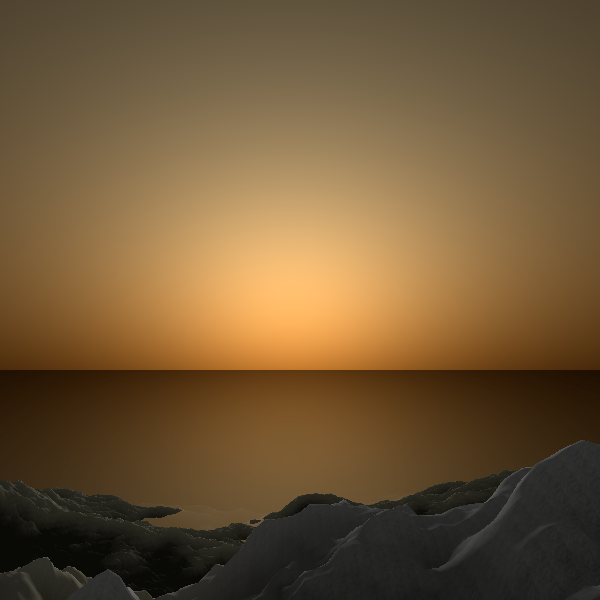
\includegraphics[scale=0.25]{scatterMie}
        \caption{Mie scattering}
        \label{fig:scatterMie}
    \end{subfigure}
    ~
    \begin{subfigure}[b]{0.45\textwidth}
        \centering
        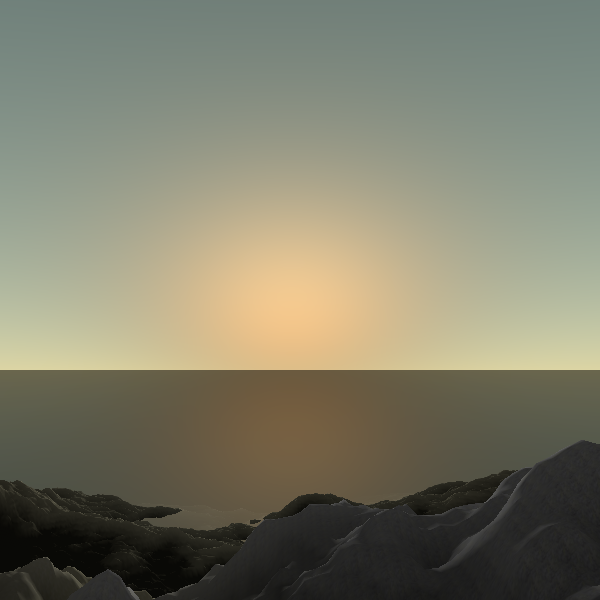
\includegraphics[scale=0.25]{scatterRayleighMie}
        \caption{Rayleigh and mie scattering}
        \label{fig:scatterRayleighMie}
    \end{subfigure}
    ~
    \begin{subfigure}[b]{0.45\textwidth}
        \centering
        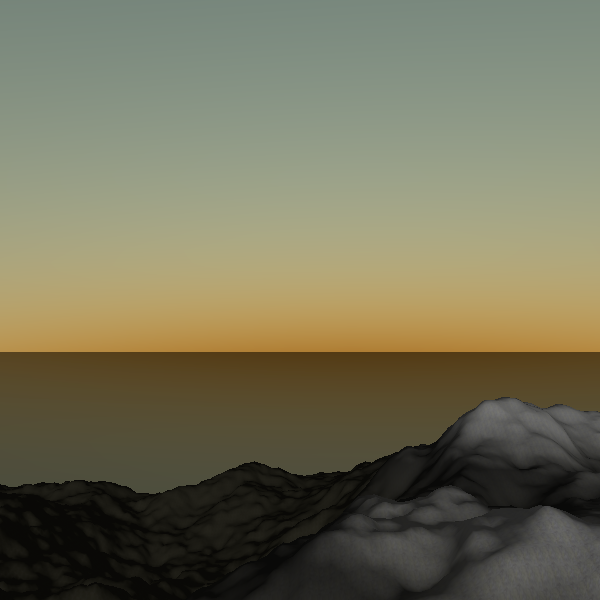
\includegraphics[scale=0.25]{scatterBack}
        \caption{Rayleigh backscattering}
        \label{fig:scatterBack}
    \end{subfigure}
    \caption{}
    \label{fig:sunScatterResults}
\end{figure}


Images showing the effect from early morning to late evening is show in figure \ref{fig:sunriseset}. As can be seen in the figures, the effect of only including the first order term in the scattering simulation during early dawn and dusk is clearly visible.

\begin{figure}[H]
\centering
    \begin{subfigure}[b]{0.45\textwidth}
        \centering
        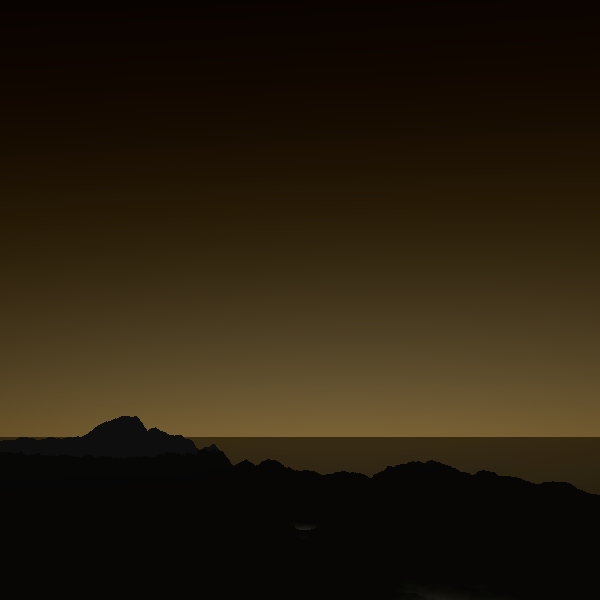
\includegraphics[scale=0.25]{light2}
        \caption{Early dawn, absence of higher order scattering terms obvious}
        \label{fig:light2}
    \end{subfigure}
    ~
    \begin{subfigure}[b]{0.45\textwidth}
        \centering
        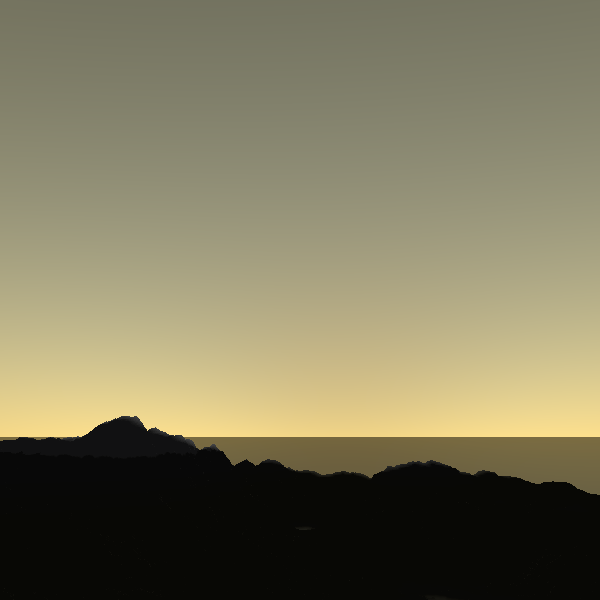
\includegraphics[scale=0.25]{light5}
        \caption{Just before sunrise}
        \label{fig:light5}
    \end{subfigure}
    ~
    \begin{subfigure}[b]{0.45\textwidth}
        \centering
        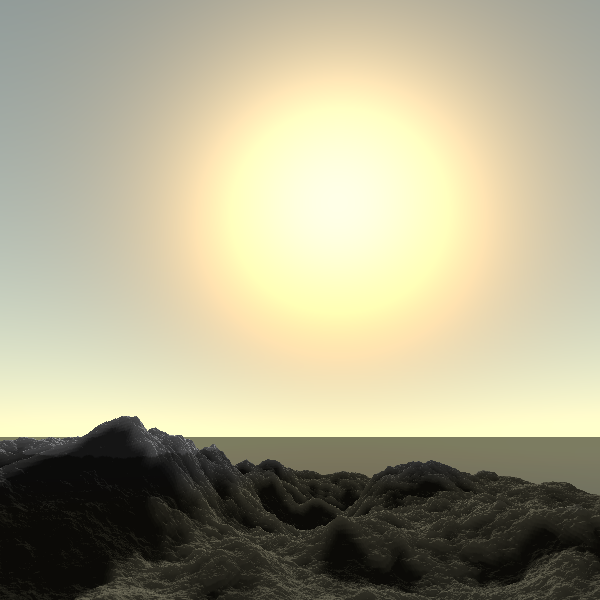
\includegraphics[scale=0.25]{light10}
        \caption{Sunrise}
        \label{fig:light7}
    \end{subfigure}
    ~
    \begin{subfigure}[b]{0.45\textwidth}
        \centering
        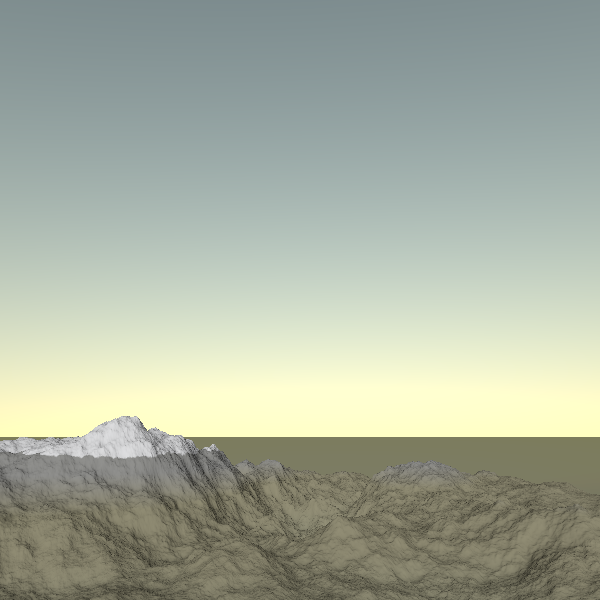
\includegraphics[scale=0.25]{light17}
        \caption{Daylight backscattering}
        \label{fig:light7}
    \end{subfigure}
    ~
    \begin{subfigure}[b]{0.45\textwidth}
        \centering
        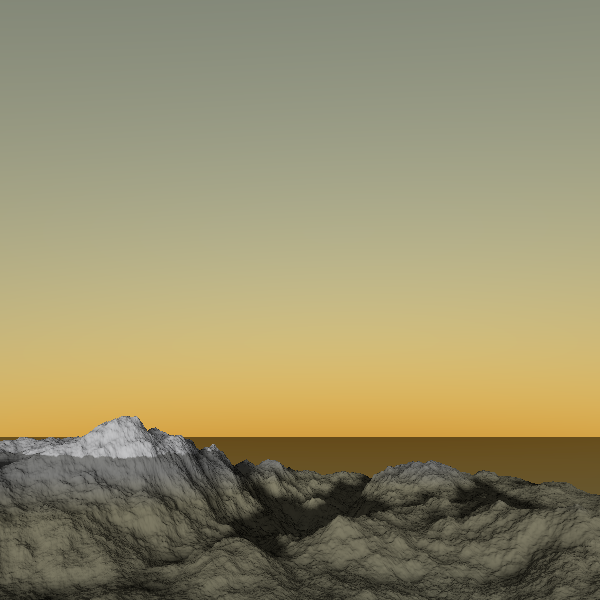
\includegraphics[scale=0.25]{light19}
        \caption{Sunset}
        \label{fig:light10}
    \end{subfigure}
    ~
    \begin{subfigure}[b]{0.45\textwidth}
        \centering
        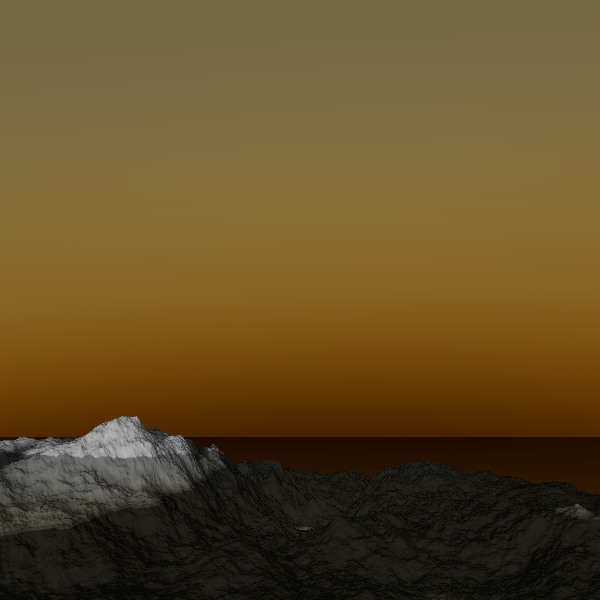
\includegraphics[scale=0.25]{light21}
        \caption{Dusk, absence of higher order scattering terms obvious}
        \label{fig:light10}
    \end{subfigure}
    \caption{}
    \label{fig:sunriseset}
\end{figure}

\subsection{Shadows}
Shadows are a very important aspect of a realistic rendering pipeline. Without the shadows the world looks weird since the human brain expects there to be shadows if there is a visible light source. Shadows are part of secondary lightning effects, that is, they are not created through direct illumination.
In general, this problem belongs the the class of rendering algorithms covering secondary lightning effects such as raytracing or radiosity,
however only looking at first order occlusion the shadow problem can be solved efficiently with polygon based methods such as shadow mapping.

Shadow mapping is an image based solution, where an orthographic camera is positioned in the direction of the light source with frustum set to cover the whole scene. The scene is rendered to a texture with depth component only. When rendering the scene, the depth map texture is sampled to determine whether the current vertex is occluded or not.

One problem with this technique is limited Z-buffer precision, and larger worlds leads to poorer shadows giving rise to a flickering effect. The problem with Z-fighting is resolved by allowing a certain margin in the decision whether a vertex is occluded or not. This however makes some obviously occluded vertices not being shadowed, so this is a trade-off parameter that needs to be tuned against specific hardware.
The other problem is aliasing: vertices far away is mapped to a single pixel in the shadow map stage, leading to jagged shadows. This problem is slightly resolved by filtering the shadows, looking in a neighborhood around each vertex, giving a smoother shadow effect. Another solution would be to increase the texture size, on the expanse of making the shadow mapping stage slower.

Results for different margins on the shadow map is shown in figures \ref{fig:shadowMapMargin}.
Results for different filter kernel sizes is shown in figures \ref{fig:shadowMapFilter}.
A combination of margin and filtering is shown in figure \ref{fig:shadowMapMarginFilter}.
The images are taken on hardware with 24 bit wide depth buffer.

\begin{figure}[H]
\centering
    \begin{subfigure}[b]{0.45\textwidth}
        \centering
        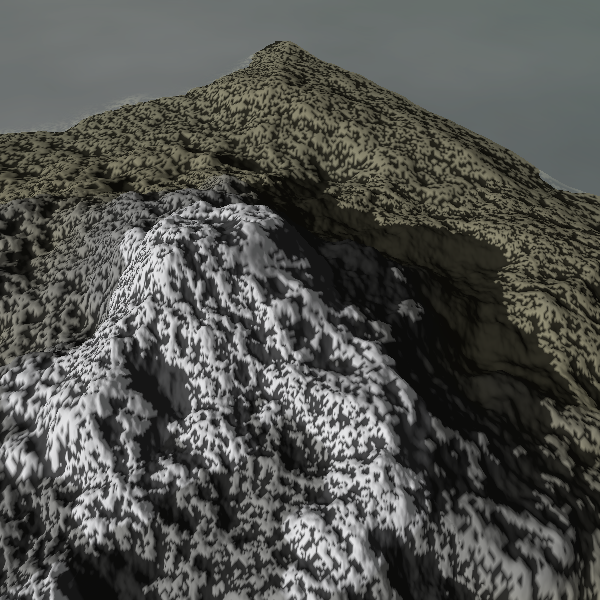
\includegraphics[scale=0.25]{shadowMargin0}
        \caption{No margin}
        \label{fig:shadowMargin0}
    \end{subfigure}
    ~
    \begin{subfigure}[b]{0.45\textwidth}
        \centering
        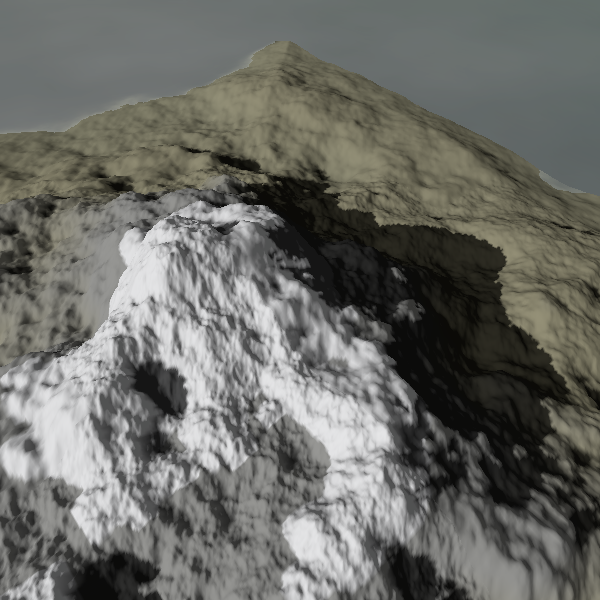
\includegraphics[scale=0.25]{shadowMargin1}
        \caption{0.01 margin}
        \label{fig:shadowMargin1}
    \end{subfigure}
    ~
    \begin{subfigure}[b]{0.45\textwidth}
        \centering
        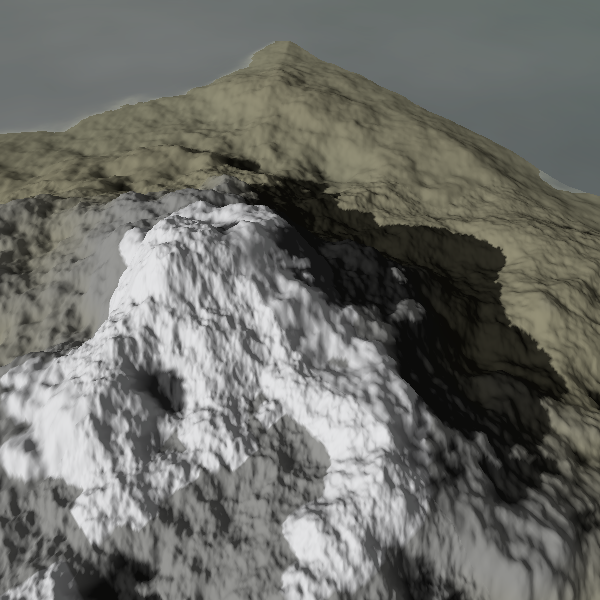
\includegraphics[scale=0.25]{shadowMargin2}
        \caption{0.02 margin}
        \label{fig:shadowMargin2}
    \end{subfigure}
    ~
    \begin{subfigure}[b]{0.45\textwidth}
        \centering
        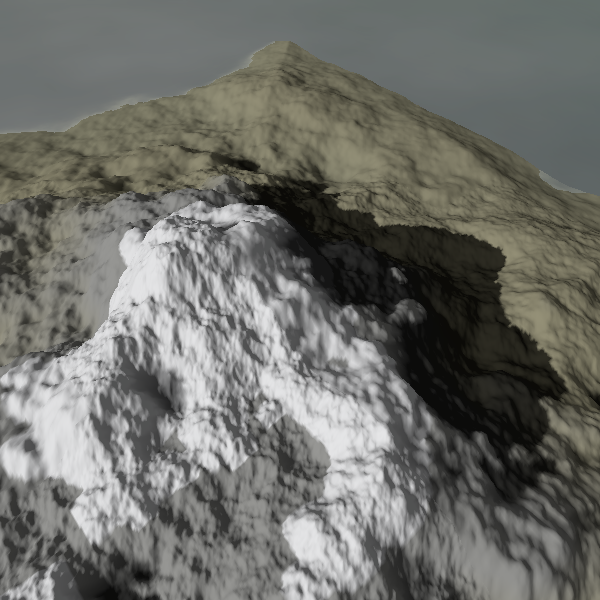
\includegraphics[scale=0.25]{shadowMargin3}
        \caption{0.03 margin}
        \label{fig:shadowMargin3}
    \end{subfigure}
    \caption{Shadow mapping with different Z-buffer margins}
    \label{fig:shadowMapMargin}
\end{figure}

\begin{figure}[H]
\centering
    \begin{subfigure}[b]{0.45\textwidth}
        \centering
        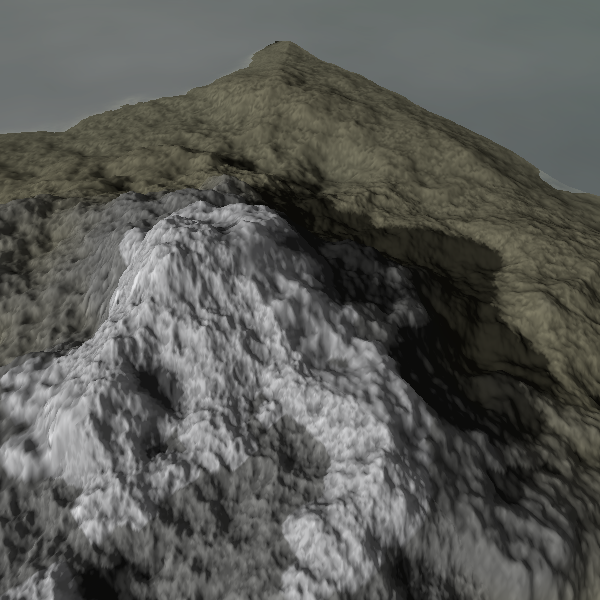
\includegraphics[scale=0.25]{shadowFilter1}
        \caption{3x3 kernel}
        \label{fig:shadowFilter1}
    \end{subfigure}
    ~
    \begin{subfigure}[b]{0.45\textwidth}
        \centering
        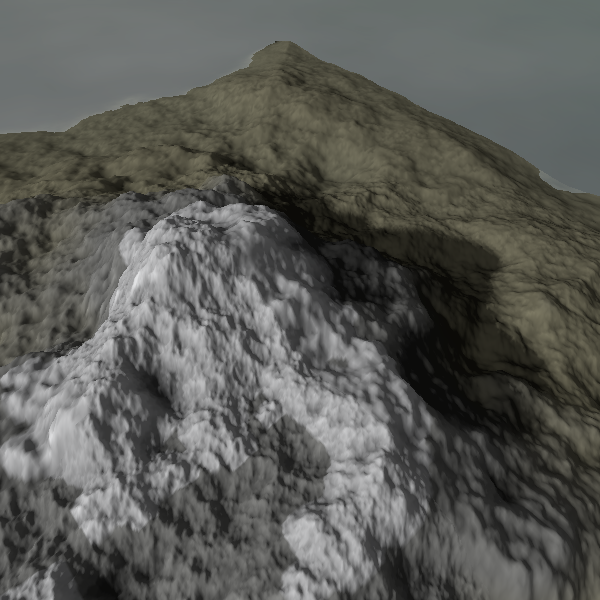
\includegraphics[scale=0.25]{shadowFilter2}
        \caption{5x5 kernel}
        \label{fig:shadowFilter2}
    \end{subfigure}
    ~
    \begin{subfigure}[b]{0.45\textwidth}
        \centering
        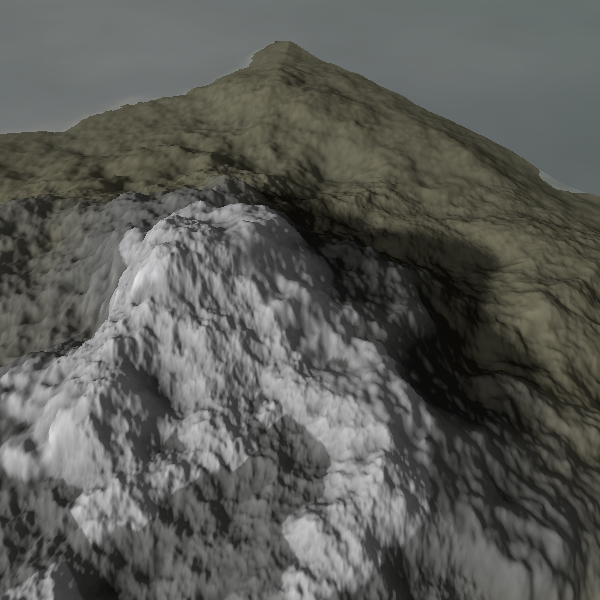
\includegraphics[scale=0.25]{shadowFilter3}
        \caption{7x7 kernel}
        \label{fig:shadowFilter3}
    \end{subfigure}
    ~
    \begin{subfigure}[b]{0.45\textwidth}
        \centering
        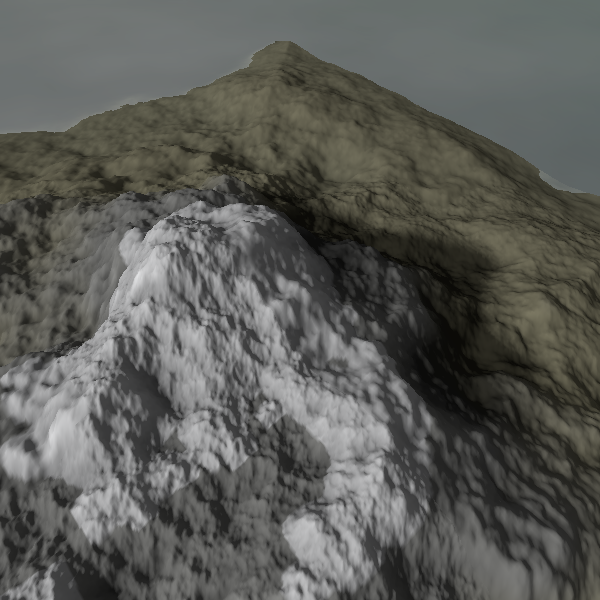
\includegraphics[scale=0.25]{shadowFilter4}
        \caption{9x9 kernel}
        \label{fig:shadowFilter4}
    \end{subfigure}
    \caption{Shadow mapping with different filter kernel sizes}
    \label{fig:shadowMapFilter}
\end{figure}

\begin{figure}[H]
\centering
    \centering
    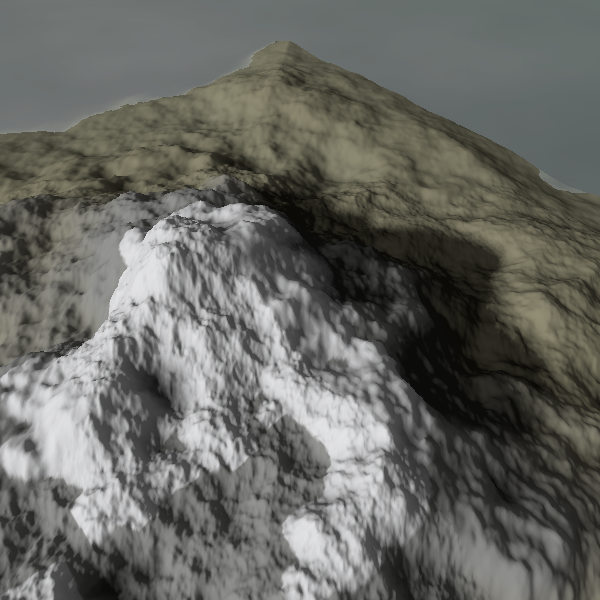
\includegraphics[scale=0.5]{shadowMargin1Filter2}
    \caption{Shadow mapping with 0.01 Z-buffer margin and 5x5 filter kernel size gives a good trade-off between rendering quality and efficiency}
    \label{fig:shadowMapMarginFilter}
\end{figure}

\subsection{Reflections}
For an open world to look open (infinite), one needs to tie together everything at the horizon.
This can be done for example by adding a water effect (an infinite, very silent sea). For this to look reasonable one needs to add reflections, otherwise the water does not look like anything.
Completely reflective water however looks unrealistic, real water is also transparent. This demands, reflectance and transparency, are non-trivial to implement (but not impossible), and this is where the stencil buffer comes to the rescue. The algorithm used for this project for rendering water is outlined below.

\begin{enumerate}\label{enum:reflectAlgo}
    \item Render original scene
    \begin{itemize}
        \item Choose water alpha level (reflectivity)
        \item Set stencil clear value to 0xFF, clear all buffers
        \item Enable depth and stencil testing
        \item Let the test stencil test always pass, replace stencil value with 0 (terrain) on depth and stencil pass
    \end{itemize}
    \item Render a plane representing the water
    \begin{itemize}
        \item Enable depth and stencil testing
        \item Let the stencil test always pass, replace with 0xFF (water) on depth and stencil pass
    \end{itemize}
    \item Bind second framebuffer with texture color attachment, render the scene upside down 
    \begin{itemize}
        \item Clear all buffers
        \item Disable stencil testing
        \item Cull front faces
    \end{itemize}
    \item Render a billboard covering the whole image, sample from the texture render target
    \begin{itemize}
        \item Enable stencil test again, let the test pass on stencil value equal to 0xFF (water but not terrain)
        \item Enable blending, let the blending function be destination alpha and one minus destination alpha (water reflectivity)
    \end{itemize}
\end{enumerate}

The results for different water transparency levels are shows in figure \ref{fig:waterAlpha}.

\begin{figure}[H]
\centering
    \begin{subfigure}[b]{0.45\textwidth}
        \centering
        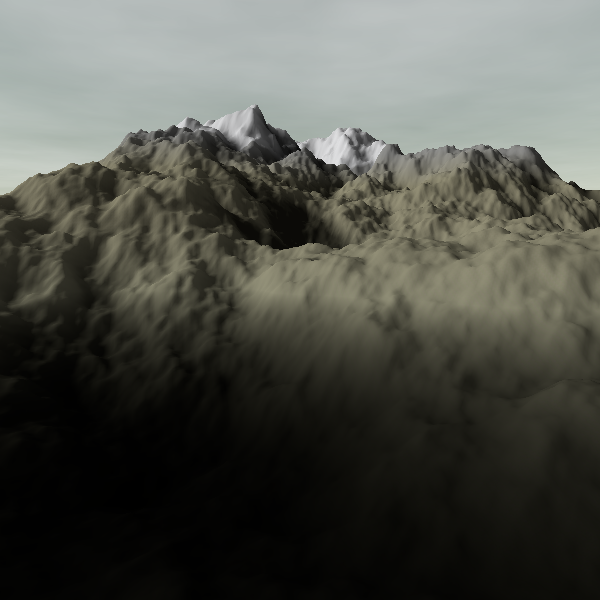
\includegraphics[scale=0.25]{waterAlpha0}
        \caption{0 alpha value}
        \label{fig:waterAlpha0}
    \end{subfigure}
    ~
    \begin{subfigure}[b]{0.45\textwidth}
        \centering
        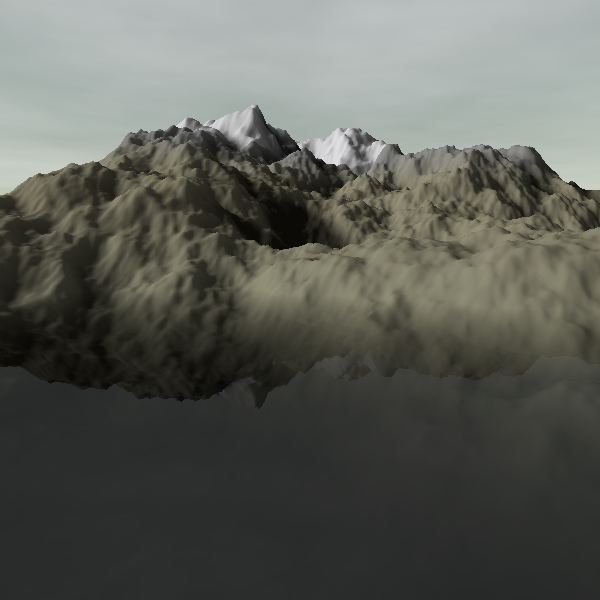
\includegraphics[scale=0.25]{waterAlpha005}
        \caption{0.05 alpha value}
        \label{fig:waterAlpha005}
    \end{subfigure}
    ~
    \begin{subfigure}[b]{0.45\textwidth}
        \centering
        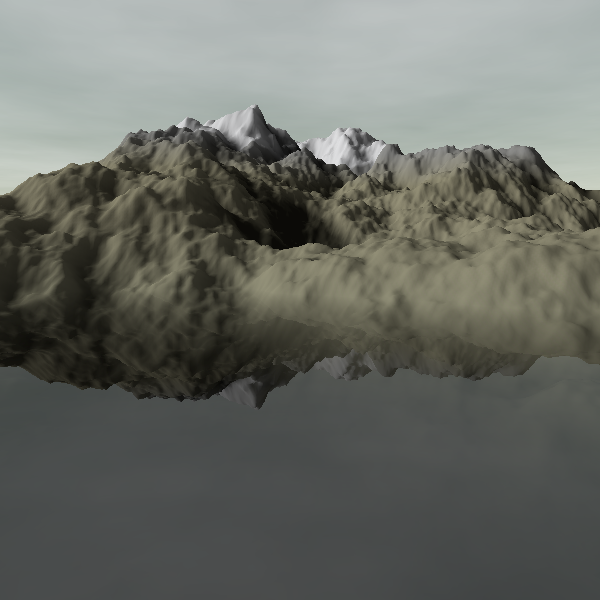
\includegraphics[scale=0.25]{waterAlpha015}
        \caption{0.15 alpha value}
        \label{fig:waterAlpha015}
    \end{subfigure}
    ~
    \begin{subfigure}[b]{0.45\textwidth}
        \centering
        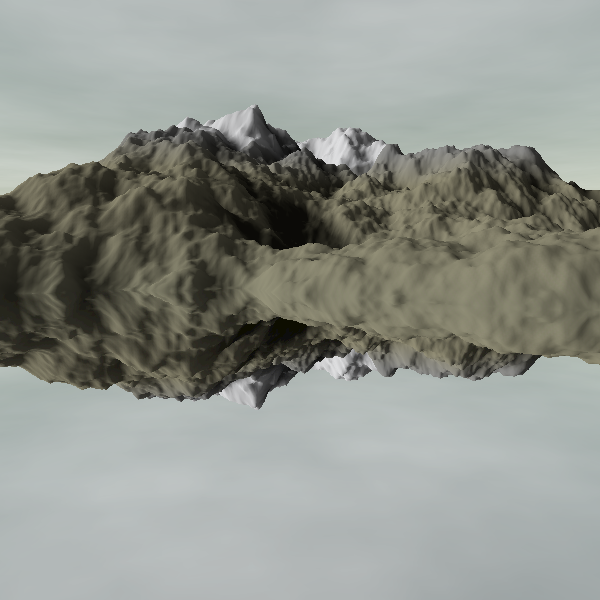
\includegraphics[scale=0.25]{waterAlpha1}
        \caption{1 alpha value}
        \label{fig:waterAlpha1}
    \end{subfigure}
    \caption{Different alpha values for the water mask determines the transparency and reflective properties}
    \label{fig:waterAlpha}
\end{figure}

\section{Particles}
We are on a mountain, but where did the snow come from?
Of course, it needs to snow, so we add a particle system!

The particle system is rendered as instanced billboards with 4 vertices. The fragment calculates the distance from the fragment to the center of the billboard, the resulting particle appears to round.
The particle system is updated with transform feedback. The transform feedback shader adds gravity, air resistance and random acceleration vectors to the particles (Brownian motion). The result is an acceptable effect of a snowfall.
The effect is shown in figure \ref{fig:snowfall}.

\begin{figure}[H]
\centering
    \centering
    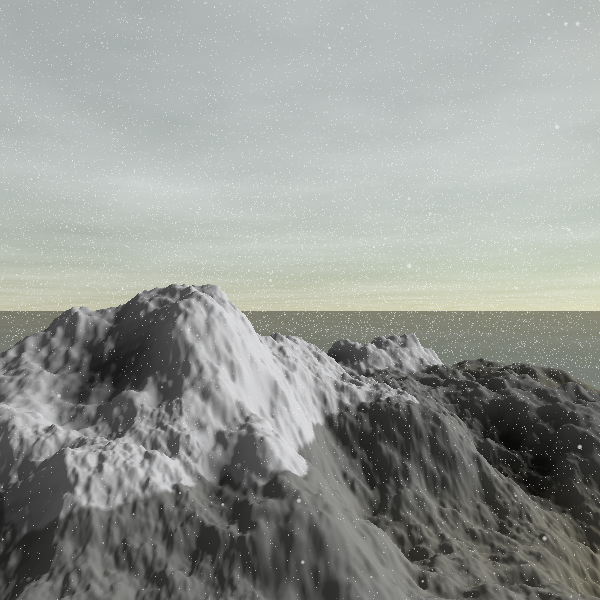
\includegraphics[scale=0.5]{snowfall}
    \caption{A snowfall effect}
    \label{fig:snowfall}
\end{figure}

\section{Problems}
The main problems encountered during the project are listed below.
\begin{itemize}
    \item Implementing edge constraints for geo-mapping seems to be impossible to in a generic way, a lot code for such a little (but nevertheless important) effect
    \item Tuning the parameters for the scattering shader was hard, and it took some while before I realized that I needed to simulate more wavelengths than just the modes of red, green and blue. The shader does not use physical constants, which would probably lead to faster tuning time for the shader.
    \item Implementing water reflectance and transparency was a bit messy using the stencil buffer approach. A more clean alternative would be to use more framebuffers to render a reflective and a transparent map separately and then blend them together.
\end{itemize}

\section{Conclusion}
All the fundamental goals of this project was completed and extended with more advanced methods.
The only limit to rendering an infinite world is memory, if the world is actually generated at different resolutions, instead of first generating full resolution and then down-sample, this could be possible. 
The biggest flaw right now is the textures, which are all of 1x1 meters. This gives rise to a highly repetitive pattern, making the scene unpleasant to look at. This could be solved by creating bigger textures, either by data collection or through some texture synthesis algorithm such as image quilting.\cite{quilt}

\printbibliography

\end{document}
